\documentclass[a4paper]{article}
\author{Simon Wehrli}
\date{30.5.2013}
\title{Set similarity with\\ b-bit k-permutation Minwise Hashing}

\usepackage[parfill]{parskip}
\usepackage{tikz} % for drawing advanced matrices
\usepackage{amsmath}
\usepackage{amssymb} % e.g. for triangle symbols
\usepackage{amsthm}
\usepackage{algorithm}
\usepackage{algorithmicx}
\usepackage{algpseudocode}
\usepackage{natbib}
\usepackage{tabulary}
\usepackage{caption}
\usepackage{framed}
\usepackage[english]{varioref} %automatische Anpassung von Referenzen
\labelformat{equation}{(#1)} %make references to equations like (1)
\usepackage{float} % bewirkt, dass Option [H] für float-Umgebungen von Latex umgesetzt wird

\usetikzlibrary{matrix,decorations.pathreplacing,backgrounds,positioning}

\DeclareMathOperator{\Var}{Var}
\DeclareMathOperator{\E}{E}

\renewcommand{\algorithmicrequire}{\textbf{Input:}}
\renewcommand{\algorithmicensure}{\textbf{Output:}}

\newtheorem{mydef}{Definition}
\newtheorem{mylemma}{Lemma}
\newtheorem{mytheorem}{Theorem}

\newcommand*{\bfrac}[2]{\genfrac{\lbrace}{\rbrace}{0pt}{}{#1}{#2}}

\begin{document} 
\maketitle

\section{Introduction}
This report is written for the seminar titled ``Algorithms for Database Systems'' at ETH Z\"{u}rich. The seminar participants read and summarize various papers, which treat solving problems in the context of Big Data, which is this year's topic. This report summarizes and explains the core concepts of \citep{LiK11} and \citep{LiOwZhang12}.

With Big Data, most problems emphasis shifts from single computational complexity to memory space usage considerations. Typically, the runtime is dominated by the time needed for memory accesses, hence the goal is to reduce the number of memory accesses. Often this is achieved by more compact data structures and at the price of less accurate result.

Many today's applications are faced with very large datasets. A common task is to find \emph{similarity} between two or several such sets. There are lots of problem solutions which use a mapping to sets of properties and then do a \emph{similarity search} on them. Fast (approximative) algorithms for this search enable improvements of many well-known algorithms, e.g. of machine learning and computer vision.

We start by explaining the original \textsc{Minwise Hashing}, which nicely presents the basic idea behind all algorithms. We move on to a major improvement, the \textsc{b-bit k-permutation Minwise Hashing}, which reduces storage at the cost of more iterations in the algorithm and is a generalization of the concept. We then present \textsc{One Permutation Hashing}, which achieves surprising accuracy using only one permutation. We focus on the concepts and algorithms and will reference to papers for applications in practice.

\subsection{Notations}

We denote by $\Omega$ the set of all possible items of the sets $S_n \subseteq \Omega$, $n = 1 \text{ to } N$. $\left| \Omega \right| = D$ is always large (e.g. $D=2^{64}$). Often we consider only two sets $S_1 = X$, $S_2 = Y$. Let $a=|X \cap Y|,$ $b=|X|-a$ and $c=|Y|-a$. Figure \vref{fig:sets} summarizes these definitions graphically.

\begin{figure}[H]
\centering
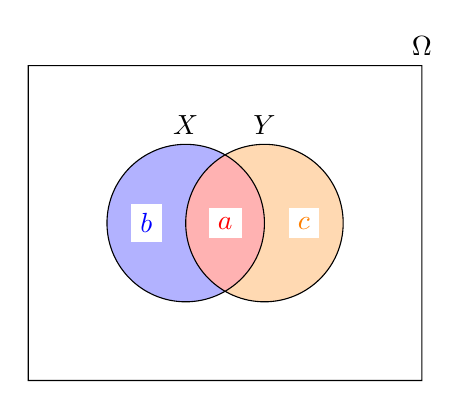
\begin{tikzpicture}
% left hand
\scope
\clip (-2,-2) rectangle (2,2)
      (1,0) circle (1);
\fill[fill=blue!30] (0,0) circle (1);
\endscope
% right hand
\scope
\clip (-2,-2) rectangle (2,2)
      (0,0) circle (1);
\fill[fill=orange!30] (1,0) circle (1);
\endscope
% middle
\scope
\clip (-2,-2) rectangle (2,2)
      (0,0) circle (1)
      (1,0) circle (1);
\fill[fill=red!30] (1,0) circle (1);
\endscope

% outline
\draw (0,0) circle (1) (0,1)  node [text=black,above] {$X$}
      (1,0) circle (1) (1,1)  node [text=black,above] {$Y$}
      (-2,-2) rectangle (3,2) node [text=black,above] {$\Omega$};
\node[draw=none,text=blue,fill=white] at (-0.5,0) {$b$};
\node[draw=none,text=red,fill=white] at (0.5,0) {$a$};
\node[draw=none,text=orange,fill=white] at (1.5,0) {$c$};
\end{tikzpicture}
\caption{Two example sets in $\Omega$ and the notation $a,b,c$ for the sizes of important subsets.}
\label{fig:sets}
\end{figure}

\paragraph{Similarity}

There exists different measurements of similarity. We will use the following throughout the paper:

\begin{framed}
\begin{mydef}\label{def:jaccard}
The normalized similarity between two sets $X$ and $Y$, known as \emph{resemblance} or \emph{Jaccard similarity}, denoted by R, is
\begin{equation}\label{eq:R}
R=\frac{\left| X \cap Y \right|}{\left| X \cup Y \right|} = \frac{a}{\left| X \right| + \left| Y \right| -a}=\frac{a}{a+b+c}
\end{equation}
\end{mydef}
\end{framed}

Another important similarity measurement is the \textit{Hamming distance}
\begin{equation}\label{eq:H}
H=\left| X \cup Y \right| - \left| X \cap Y \right| = \left| X \right| + \left| Y \right| -2a.
\end{equation}
Luckily, there is a direct transformation from one measurement to the other, by solving \vref{eq:R} after $a$ and inserting into \vref{eq:H}:
\begin{equation}
H= \left| X \right| + \left| Y \right| -2 \frac{R}{1+R} \left( |X| + |Y| \right) = \frac{1-R}{1+R} \left( |X| + |Y| \right).
\end{equation}

\paragraph{Probability}
 
Later we often look at some important event of a problem where we use $\Pr[\cdot]$ as a shorthand for the \emph{Probability} of that event. To get an estimator for $R$ out of a probabilistic argument, we always use some Bernoulli experiment. This is a process, where we repeatedly flip a possibly biased coin, but the bias does not change. We can see it as a sequence of binary random variables, because only two outcomes are possible, $0$ or $1$. An event is described by an equation. We use the notation $1\left\lbrace \text{\textit{equation}} \right\rbrace$ which is one if and only if the \textit{equation} in curly braces is true:
\begin{equation*}
1\left\lbrace \text{\textit{equation}} \right\rbrace =\begin{cases}
    1 & \text{if \textit{equation} evaluates to \textit{true}} \\
    0 & \text{otherwise}
\end{cases}
\end{equation*}

\paragraph{Runtime/Storage Analysis}

When we do the analysis of an algorithm, we use the big-$O$-notation. For storage requirement analysis we count in bits, because we later do optimizations on the bit level. This belongs to the \textit{logarithmic cost model}. Contrary, for runtime analyses we count in the \textit{uniform cost model}, thus each operation needs one unit of time. Especially for comparison operations of set elements, we assume that the binary representation always fits a 64-bit integer. This is equal to the realistic assumption that $D <= 2^{64}$.

\subsection{Motivating Example}
Consider a web search provider, which want to present a result list of web pages without duplicates. To achieve that, for every pair of web pages, we drop one of them, if they are textually very similar. This is the case when their \emph{resemblance} $R$ is greater than some threshold $R_0$. But to be able to use the \emph{resemblance} as a measurement, we have to map each page to a set. One could imagine to define this mapping from the page to the set of all words occurring on that page. But with this mapping would not keep track of the order in which their appear. As in several studies \citep{Broder:1998,BroderGMZ97} we will instead map a page to a set of \emph{shingles}. A shingle is a string of $w$ contiguous words, and we include a \emph{shingle} in our result set if the \emph{shingle} occurs on the page (in the same order). Typically we choose $w = 5$. Figure \vref{fig:shingle} shows an exemplary mapping.

\begin{figure}[H]
\begin{center}
\fbox{
\parbox{2cm}{
This web page is just an example.
}
}
\hspace{1cm} $\underrightarrow{\text{mapping}}$ \hspace{1cm}
\parbox{2cm}{
\begin{equation*}
\begin{split}
 \text{\{} & \text{``This web page''},\\ & \text{``web page is''},\\ & \text{``page is just''},\\ & \text{``is just an''},\\ & \text{``just an example''} \text{\}}
\end{split}
\end{equation*}
}
\end{center}
\caption{The mapping from a web page to a set of \emph{shingles}.}
\label{fig:shingle}
\end{figure}

Clearly, the number of possible shingles and therefore $D$ is huge. Assuming $10^5$ different English words, we have $D=\left(10^5\right)^5 \gg 2^{64}$. Thus computing the exact similarities for all pairs of pages of a web search would require prohibitive storage. In general we would already need $\Theta(D)$ storage for a single pair. We need approximation algorithms to improve significantly on this bound.

However, finding duplicates out of $m$ objects, e.g. web pages, needs $O(m^2)$ comparisons even when approximating the similarity. This is a different problem and there are a  number of approaches to deal with it, but we will not discuss it here and refer to \citep{BroderGMZ97,STOC02*380}.

\section{Original Minwise Hashing}

A working approximative solution to this problem was described by Broder and his colleagues \citep{Broder:1998,BroderGMZ97}. We demonstrate their algorithm on a small running example. Suppose we have two web pages $P_X$ and $P_Y$ and want to compare them:

\begin{figure}[H]
\begin{center}
\fbox{
\parbox{2cm}{
u v u v
}
}
\hspace{1cm} $\underleftrightarrow{\text{similar?}}$ \hspace{1cm}
\fbox{
\parbox{2cm}{
w v u
}
}
\end{center}
\end{figure}

We map both pages to sets of length-$2$-shingles. So $P_X$ becomes $\{ \text{``uv''}, \text{``vu''} \}$ and $P_Y$ becomes $\{ \text{``wv''}, \text{``vu''} \}$. Note that the mapping is indifferent to that ``uv'' occurs twice on $P_X$. When we continuously  number all possible shingles $\{ \text{``uu''}, \text{``uv''}, \text{``uw''}, \text{``vu''}, \text{``vv''}, \text{``vw''}, \text{``wu''}, \text{``wv''}, \text{``ww''} \}$ and define this to be $\Omega_{\text{shingle}}$, we can visualize sets in a binary matrix
\begin{equation*}
M \in \{ 0,1 \}^{N \times D}, \qquad M_{ni}=1\left\lbrace i \in S_n \right\rbrace.
\end{equation*}

Applied to our example, we get

\begin{equation}
M= 
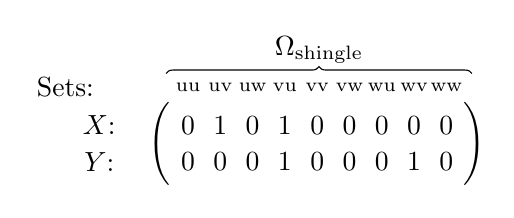
\begin{tikzpicture}[baseline = (M.center),% center with respect to the matrix center
        every left delimiter/.style={xshift=1ex},%tighter delimiter spacing
        every right delimiter/.style={xshift=-1ex}]
\matrix (M) [matrix of math nodes,left delimiter={(},right delimiter={)} 
        ]{ 
0&1&0&1&0&0&0&0&0\\
0&0&0&1&0&0&0&1&0\\
};
\node[anchor=south east] (cornernode) at (M-1-1.north west) {Sets: \qquad \qquad}; %Position this more precisely if desired
\foreach[count=\xi] \x in {uu,uv,uw,vu,vv,vw,wu,wv,ww}{ %\xi is the counter \x is the value
\node[font=\scriptsize] (M-0-\xi) at (cornernode -| M-1-\xi) {\x}; % Gets the top row 
 }

\foreach[count=\xi] \x in {$X$:,$Y$:}{ %\xi is the counter \x is the value
\node (M-\xi-0) at (cornernode |- M-\xi-1) {\x}; %Gets the left most column
}

\draw[decoration=brace,decorate] (M-0-1.north west) -- (M-0-9.north east)%
 node[midway,above] {$\Omega_{\text{shingle}}$};

\end{tikzpicture}
.
\end{equation}

Because working with an $\Omega_{\text{shingle}}$ of strings is nasty, we assume there is a perfect hash function applied to the elements of the original domain which always gives us $\Omega = \{0,1,\ldots,D-1\}$. Additionally we colour the columns of the matrix according to the three coloured subsets in Figure \vref{fig:sets}, e.g. a column with both entries equals to one represents an element contained in both sets. $M$ is rewritten with the new $\Omega$ as

\begin{equation}
M= 
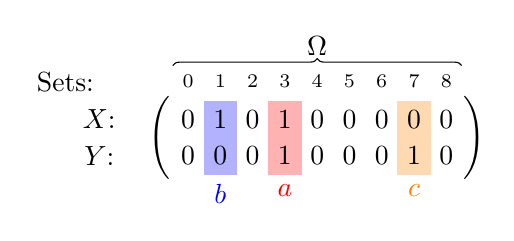
\begin{tikzpicture}[baseline = (M.center),% center with respect to the matrix center
        every left delimiter/.style={xshift=1ex},%tighter delimiter spacing
        every right delimiter/.style={xshift=-1ex}]
\matrix (M) [matrix of math nodes,left delimiter={(},right delimiter={)} 
        ]{ 
0&1&0&1&0&0&0&0&0\\
0&0&0&1&0&0&0&1&0\\
};
\node[anchor=south east] (cornernode) at (M-1-1.north west) {Sets: \qquad \qquad}; %Position this more precisely if desired
\foreach[count=\xi] \x in {0,1,2,3,4,5,6,7,8}{ %\xi is the counter \x is the value
\node[font=\scriptsize] (M-0-\xi) at (cornernode -| M-1-\xi) {\x}; % Gets the top row 
 }

\foreach[count=\xi] \x in {$X$:,$Y$:}{ %\xi is the counter \x is the value
\node (M-\xi-0) at (cornernode |- M-\xi-1) {\x}; %Gets the left most column
}

\node[color=blue, below = 0.1pt of M-2-2.south] {$b$};
\node[color=red, below = 0.1pt of M-2-4.south] {$a$};
\node[color=orange, below = 0.1pt of M-2-8.south] {$c$};

\draw[decoration=brace,decorate] (M-0-1.north west) -- (M-0-9.north east)%
 node[midway,above] {$\Omega$};

\begin{scope}[on background layer]
\draw [draw=none, fill=blue!30] (M-1-2.north west) rectangle (M-2-2.south east);
\draw [draw=none, fill=red!30] (M-1-4.north west) rectangle (M-2-4.south east);
\draw [draw=none, fill=orange!30] (M-1-8.north west) rectangle (M-2-8.south east);
\end{scope}

\end{tikzpicture}
.
\end{equation}


For reasons which later become clear, suppose a random permutation $\pi$ is performed on $\Omega$,
\begin{equation*}
\pi:\Omega \longrightarrow \Omega.
\end{equation*}


To simplify notation, we overload the definition of $\pi$ to work also for subsets of $\Omega$. Thus with $\pi(S_n)$ we denote the application of the permutation $\pi$ to every element of the set $S_n$. More precisely,
\begin{equation*}
\begin{split}
\pi &: 2^\Omega \longrightarrow 2^\Omega, \\
\pi &: S_n \longmapsto \pi \left( S_n \right) = \left\lbrace \pi \left( i \right) \middle\vert i \in S_n \right\rbrace. 
\end{split}
\end{equation*}

In the matrix representation, the application of $\pi$ can be seen as rearranging the matrix columns in a random order. For an exemplary chosen $\pi$ this could look like

\begin{equation}
M'= 
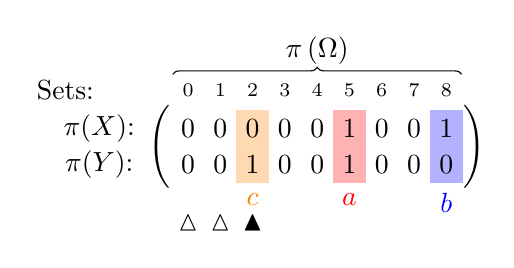
\begin{tikzpicture}[baseline = (M.center),% center with respect to the matrix center
        every left delimiter/.style={xshift=1ex},%tighter delimiter spacing
        every right delimiter/.style={xshift=-1ex}]
\matrix (M) [matrix of math nodes,left delimiter={(},right delimiter={)} 
        ]{ 
0&0&0&0&0&1&0&0&1\\
0&0&1&0&0&1&0&0&0\\
};
\node[anchor=south east] (cornernode) at (M-1-1.north west) {Sets: \qquad \qquad}; %Position this more precisely if desired
\foreach[count=\xi] \x in {0,1,2,3,4,5,6,7,8}{ %\xi is the counter \x is the value
\node[font=\scriptsize] (M-0-\xi) at (cornernode -| M-1-\xi) {\x}; % Gets the top row 
 }

\foreach[count=\xi] \x in {$\pi(X)$:,$\pi(Y)$:}{ %\xi is the counter \x is the value
\node (M-\xi-0) at (cornernode |- M-\xi-1) {\x}; %Gets the left most column
}

\node[color=blue, below = 0.1pt of M-2-9.south] {$b$};
\node[color=red, below = 0.1pt of M-2-6.south] {$a$};
\node[color=orange, below = 0.1pt of M-2-3.south] {$c$};

\draw[decoration=brace,decorate] (M-0-1.north west) -- (M-0-9.north east)%
 node[midway,above] {$\pi\left(\Omega \right)$};

\begin{scope}[on background layer]
\draw [draw=none, fill=blue!30] (M-1-9.north west) rectangle (M-2-9.south east);
\draw [draw=none, fill=red!30] (M-1-6.north west) rectangle (M-2-6.south east);
\draw [draw=none, fill=orange!30] (M-1-3.north west) rectangle (M-2-3.south east);
\end{scope}


\node[below = 8pt of M-2-1.south] {$\vartriangle$};
\node[below = 8pt of M-2-2.south] {$\vartriangle$};
\node[below = 8pt of M-2-3.south] {$\blacktriangle$};

\end{tikzpicture}
.
\end{equation}

Suppose now there is a pointer $\blacktriangle$ starting at the left most column of $M'$, moving to the right until it sees the first column where there is at least one $1$ (i.e. skip columns of only zeros). In our example $\blacktriangle$ would stop at index $2$. We can define the event $\omega$, that $\blacktriangle$ stops at a column with two ones, which corresponds to the subset $a$. We ask for the probability of $\omega$ and find
\begin{equation*}
\Pr \left[ \blacktriangle \text{ stops at } \left(
\begin{array}{c}
1  \\
1  \end{array}
\right) \right] = \Pr \left[ \omega \right] = \frac{a}{a+b+c} = R,
\end{equation*}

because we randomly permuted the columns.
To determine if or if not $\omega$ arises for the given permutation $\pi$, we only need the index of the left most $1$ in each row respectively the smallest element of each set $S_n$ permuted with $\pi$. We define this smallest element of the permuted set\footnote{Note that the smallest element changes under the permutations because $\pi$ is a permutation on $\Omega$ and $S_n$ is only a subset of $\Omega$ in general.} as
\begin{equation}
h_{S_n,\pi}=min(\pi(S_n)).\footnote{The denotation $h$ is choosen, because the mapping can be interpreted as a hash function with desired properties for similarity estimation.}
\end{equation}


This key observation leads to the crucial

\begin{framed}
\begin{mylemma} \label{lem:minwiseHashing}
For any two sets $X,Y \subseteq \Omega$
\begin{equation}\label{eq:minwiseOri}
\Pr [\min(\pi(X))=\min(\pi(Y))]=\Pr[h_{X,\pi}=h_{Y,\pi}]=\frac{\left| X \cap Y \right|}{\left| X \cup Y \right|}=R.
\end{equation}
\end{mylemma}
\end{framed}


To estimate $R$ via a \textit{Bernoulli Process} we must evaluate $\omega$ not only once but on $k$ independent random permutations $\pi_1,\pi_2,\ldots,\pi_k$. By averaging the outcomes we finally build the estimator
\begin{equation}\label{eq:minwiseEstimator}
\hat{R}_M=\frac{1}{k}\sum_{j=1}^k 1 \left\lbrace h_{X,\pi_j}=h_{Y,\pi_j} \right\rbrace,
\end{equation}
\begin{equation}\label{eq:minWiseVariance}
Var(\hat{R}_M)=\frac{1}{k}R(1-R).
\end{equation}

It can be proven, that $\E(Var(\hat{R}_M)) = R$ which means that the estimator is unbiased.
We later refer to $h_{S_n,\pi_j}$ as a \textbf{sample} and to $k$ as the \textbf{sample size}. Note that we only have to store a \textbf{sample} for each permutation and this for each set. But we can reuse the same $k$ permutations for all sets and precompute the $k$ \textbf{samples} for each set individually.

The minimum function $\min(\cdot)$ needs $O(D)$ time. For a similarity calculation of two specific sets we then only have to make the computations from \vref{eq:minwiseEstimator}, thus $O(k)$ steps. Altogether we learn that the algorithm has to consist of two phases, the pre-processing and the similarity calculation.
For the pre-processing especially the storage requirement of the samples is relevant. Each sample potentially needs $O(\log(D))$ bits, because the smallest element can be any element in $D$. By using $k$ permutations, we need $O(k \log(D))$ bits in total.

Many applications, especially duplicate detection tools, are interested in detecting somewhat high similarity, thus an approximation seems reasonable. From \vref{eq:minWiseVariance} we learn, that the accuracy can be adjusted by choosing the \textbf{sample size} appropriately. In practice we typically have a $k$ between $2^5$ to $2^8$. Even though $k$ can be considered as a constant, the storage requirement of the pre-processing often gets impractical.



\subsection{The Algorithm}

Based on the theoretical results, Algorithm \vref{alg:orgMinwiseHashing} presents the procedure of ($k$-permutation) \textsc{Minwise Hashing}.

\begin{algorithm}[H]
\caption{Original \textsc{Minwise Hashing} algorithm, applied to estimating pairwise resemblances in a collection of $N$ sets.}
\label{alg:orgMinwiseHashing}
\begin{algorithmic}
\Require Sets $S_n \subseteq \Omega = \{0,1,\ldots,D-1\}, n = 1 \text{ to } N$. \Comment $D = \left| \Omega \right|$
\Ensure Estimated resemblance $\hat{R}_M$
\State // Pre-processing
\State Generate $k$ random permutations $\pi_j: \Omega\longrightarrow\Omega, j=1\text{ to }k$
\ForAll{$n = 1 \text{ to } N, j = 1 \text{ to } k$}
	\State Store $\min(\pi_j(S_n))$, denoted by $h_{S_n,\pi_j}$.
\EndFor
\State
\State // Estimation (Use two sets $X,Y$ as an example)
\State Estimate the resemblance by $\hat{R}_M=\frac{1}{k}\sum_{j=1}^k 1 \left\lbrace h_{X,\pi_j}=h_{Y,\pi_j} \right\rbrace$
\end{algorithmic}
\end{algorithm}





\section{b-bit k-permutation Minwise Hashing}\label{sec:b-bitMinwiseHashing}

We will present an algorithm which improves on the storage requirements of the original \textsc{Minwise Hashing}. The idea is to reduce the size of each \textbf{sample} by only taking $b$ bits of it, as opposed to, e.g. $64$ bits. Intuitively, this will increase the estimation variance $Var(\hat{R}_M)$, at the same \textbf{sample size} $k$. To maintain the same accuracy, we have to increase $k$. One can show, if the resemblance is not too small, we will not have to increase $k$ much and in total use less storage.

For example, when $b=1$ and $R=0.5$, the estimation variance will increase at most by a factor of $3$. To keep the same accuracy, we have to increase the \textbf{sample size} by a factor of $3$. If we before stored each minimum $\min(\pi_j(S_n))$ using $64$ bits, the improvement with $b=1$ is $64/3=21.3$.

Consider again two sets $X,Y \subseteq \Omega$, on which a random permutation $\pi: \Omega \longrightarrow \Omega$ is applied. We extend our notation with
\[
h_{X,b,\pi}=b \text{ lowest bits of } \min(\pi(X))
\]
\[
h_{Y,b,\pi}=b \text{ lowest bits of } \min(\pi(Y))
\]
\begin{framed}
\begin{mytheorem} \label{the:b-bitMinwiseHashing}
Assume $D$ is large.
\begin{equation}\label{eq:minwiseB-bit}
P_b=\Pr[1\left\lbrace h_{X,b,\pi}=h_{Y,b,\pi}\right\rbrace]=C_{1,b}+(1-C_{2,b})R
\end{equation}
\begin{equation}
r_X=\frac{|X|}{D}, \qquad r_Y=\frac{|Y|}{D}
\end{equation}
\begin{equation}
\begin{split}
C_{1,b}=A_{X,b}\frac{r_Y}{r_X+r_Y}+A_{Y,b}\frac{r_X}{r_X+r_Y},\\
C_{2,b}=A_{X,b}\frac{r_X}{r_X+r_Y}+A_{Y,b}\frac{r_Y}{r_X+r_Y}
\end{split}
\end{equation}
\begin{equation}
A_{X,b}=\frac{r_X[1-r_X]^{2^b-1}}{1-[1-r_X]^{2^b}}, \qquad A_{Y,b}=\frac{r_Y[1-r_Y]^{2^b-1}}{1-[1-r_Y]^{2^b}}
\end{equation}
\end{mytheorem}
\end{framed}

The intuition for the additional terms $C_{1,b}$ and $C_{2,b}$ in \vref{eq:minwiseB-bit} compared to \vref{eq:minwiseOri} is that we have to account for a type of ``false positive'': When two minima agree on their last $b$ bits, $h_{X,b,\pi}=h_{Y,b,\pi}$, it's still possible that their are different, $h_{X,\pi}\neq h_{Y,\pi}$. Thus even when $R=0$, the collision probability $P_b$ is not zero, but rather $C_{1,b}$. This makes the derivation much more complicated.\footnote{A proof of Theorem \vref{the:b-bitMinwiseHashing} can be found in the appendix of \citep{LiK09}.}

Even though $D$ is assumed to be large, experiments show that even for $D=20$ the absolute error caused by using \vref{eq:minwiseB-bit} ist $< 0.01$.

\subsection{The Estimator}

From \vref{eq:minwiseB-bit} of Theorem \vref{the:b-bitMinwiseHashing} we derive the estimator $\hat{R}_b$ for $R$:
\begin{equation}
\hat{R}_b=\frac{\hat{P}_b-C_{1,b}}{1-C_{2,b}}
\end{equation}
\begin{equation}
\hat{P}_b = \frac{1}{k}\sum_{j=1}^k 1 \left\lbrace  h_{X,b,\pi_j } = h_{Y,b,\pi_j } \right\rbrace
\end{equation}

This estimator is unbiased, i.e. $\E[\hat{R}_b]=R$. Furthermore, the variance of $\hat{R}_M$ converges to the variance of $\hat{R}_b$, i.e.
\begin{equation}
\lim_{b\rightarrow\inf}\Var\left(\hat{R}_b\right)=\frac{R(1-R)}{k}=\Var\left(\hat{R}_M\right)
\end{equation}

\subsection{The Algorithm}

Based on the theoretical results, Algorithm \vref{alg:minwiseHashing} presents the procedure of $b$-bit ($k$-permutation) \textsc{Minwise Hashing}.

\begin{algorithm}[H]
\caption{\textsc{b-bit Minwise Hashing} algorithm, applied to estimating pairwise resemblances in a collection of $N$ sets.}
\label{alg:minwiseHashing}
\begin{algorithmic}
\Require Sets $S_n \subseteq \Omega = \{0,1,\ldots,D-1\}, n = 1 \text{ to } N$. \Comment $D = \left| \Omega \right|$
\Ensure Estimated resemblance $\hat{R}_b$
\State // Pre-processing
\State Generate $k$ random permutations $\pi_j: \Omega\longrightarrow\Omega, j=1\text{ to }k$
\ForAll{$n = 1 \text{ to } N, j = 1 \text{ to } k$}
	\State Store the lowest $b$ bits of $\min(\pi_j(S_n))$, denoted by $h_{S_n,b,\pi_j}$.
\EndFor
\State
\State // Estimation (Use two sets $X,Y$ as an example)
\State Compute $\hat{P}_b = \frac{1}{k}\sum_{j=1}^k 1 \left\lbrace  h_{X,b,\pi_j } = h_{Y,b,\pi_j } \right\rbrace$
\State Estimate the resemblance by $\hat{R}_b = \frac{\hat{P}_b-C_{1,b}}{1-C_{2,b}}$, where $C_{1,b}$ and $C_{2,b}$ are from Theorem \vref{the:b-bitMinwiseHashing}
\end{algorithmic}
\end{algorithm}


\subsection{Deriving the Hamming Distance} \label{sec:hammingDistance}

Another well-known measurement for the similarity is the \emph{hamming distance}. For the purpose of calculating the \emph{hamming distance} between two sets $X,Y \subseteq \Omega = \{0,1,\ldots,D-1\}$, the sets are first mapped to a $D$-dimensional binary vector $x,y$ resp.:
\begin{framed}
\begin{mydef}\label{def:hamming}
Let vector $x,y \in \left\lbrace 0,1 \right\rbrace ^D, \, x_i = 1\left\lbrace i \in X \right\rbrace, y_i = 1\left\lbrace i \in Y \right\rbrace$. The \emph{hamming distance} between $X$ and $Y$ is
\begin{equation}
H=\sum_{i=0}^{D-1}\left[ x_i \neq y_i \right]=|X \cup Y|-|X\cap Y|=|X|+|Y|-2a
\end{equation}
\end{mydef}
\end{framed}

If we reformulate \vref{def:jaccard} as
\begin{equation}
a=\frac{R}{1+R}(|X|+|Y|),
\end{equation}
we can use the \textsc{b-bit Minwise Hashing} algorithm to estimate $H$ with
\begin{equation}
\hat{H}_b=|X|+|Y|-2\frac{\hat{R}_b}{1+\hat{R}_b}(|X|+|Y|)=\frac{1-\hat{R}_b}{1+\hat{R}_b}(|X|+|Y|)
\end{equation}

Experiments show that this approach is significantly faster than standard methods for computing the \emph{hamming distance}.

\subsection{Drawbacks} \label{sec:b-bitDrawbacks}

The major problem of \textsc{b-bit Minwise Hashing} is the costly preprocessing. Consider an application in machine learning, where the sets $S_n$ represents some properties of an object (e.g. a document or an image). Often one wants to add objects dynamically at runtime and compare them to other objects by finding the \emph{resemblance} of their properties. Finding the $k$ minima under the permutations may take too long, i.e. uses $O(k|S_n|)$ to $O(kD)$ time per set.
In general, the costly preprocessing may cause problems in user-facing applications, where the testing efficiency for new data objects is crucial. There is the need for a entirely fast algorithm to keep this applications responsive.

Another drawback is that storing $k$ permutations is sometimes impractical. If e.g. $D=10^9$, one permutation vector uses $4$GB, which is still possible to store. But the space needed to store e.g. $k=500$ permutation vectors (each of length $D$), is not tolerable.



\section{One Permutation Hashing}

This algorithm is directly motivated by the optimization potential of the standard \textsc{Minwise Hashing} method: intuitively, it ought to be ``wasteful'' in that all elements in a set are permuted, scanned but only the minimum will be used. As the name already suggests, we reduce the preprocessing step to only one permutation.

As in section \vref{sec:hammingDistance} we will represent sets $S_n \subseteq \Omega$ as vectors $s_n \in \left\lbrace 0,1 \right\rbrace ^D, \, (s_n)_i = 1\left\lbrace i \in S_n \right\rbrace$. We will setup a running example with $X,Y,Z \subseteq \Omega = \left\lbrace 0,1,\cdots,15\right\rbrace$. Let be $\pi$ some random permutation on $\Omega$ and the already permuted sets be
\[
\pi(X)=\left\lbrace 2,4,7,13\right\rbrace, \quad \pi(Y)=\left\lbrace 0,3,6,13\right\rbrace,\quad \pi(Z)= \left\lbrace 0,1,10,12\right\rbrace.
\]
Now again we build up a data matrix where the rows are equal to the vector representations of the permuted sets:

\begin{equation}
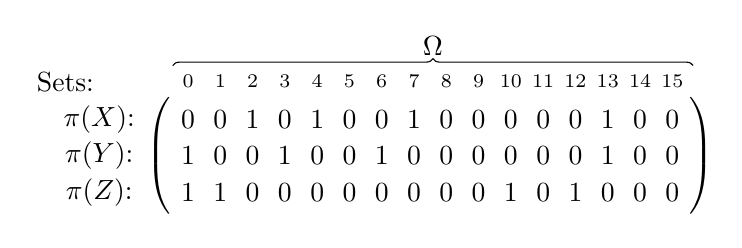
\begin{tikzpicture}[baseline = (M.center),% center with respect to the matrix center
        every left delimiter/.style={xshift=1ex},%tighter delimiter spacing
        every right delimiter/.style={xshift=-1ex}]
\matrix (M) [matrix of math nodes,left delimiter={(},right delimiter={)} 
        ]{ 
0&0&1&0&1&0&0&1&0&0&0&0&0&1&0&0\\
1&0&0&1&0&0&1&0&0&0&0&0&0&1&0&0\\
1&1&0&0&0&0&0&0&0&0&1&0&1&0&0&0\\
};
\node[anchor=south east] (cornernode) at (M-1-1.north west) {Sets: \qquad \qquad}; %Position this more precisely if desired
\foreach[count=\xi] \x in {0,1,2,3,4,5,6,7,8,9,10,11,12,13,14,15}{ %\xi is the counter \x is the value
\node[font=\scriptsize] (M-0-\xi) at (cornernode -| M-1-\xi) {\x}; % Gets the top row 
}

\foreach[count=\xi] \x in {$\pi(X)$:,$\pi(Y)$:,$\pi(Z)$:}{ %\xi is the counter \x is the value
\node (M-\xi-0) at (cornernode |- M-\xi-1) {\x}; %Gets the left most column
}

\draw[decoration=brace,decorate] (M-0-1.north west) -- (M-0-16.north east)%
 node[midway,above] {$\Omega$};

\end{tikzpicture}
\end{equation}

The idea is to divide the columns evenly into $t$ (here $t=4$) bins (parts), take the minimum in each bin. Because later we only compare minima within one bin, we can re-index the elements to use the smallest possible representation:

\begin{equation} \label{matrix:complete}
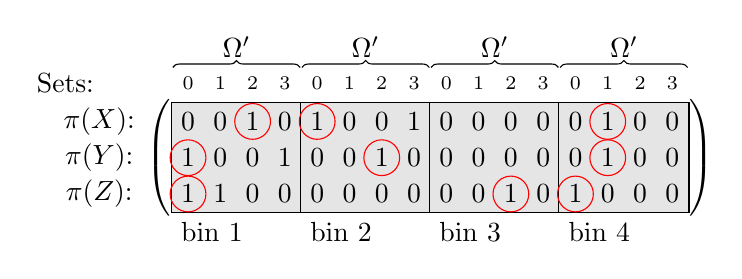
\begin{tikzpicture}[baseline = (M.center),% center with respect to the matrix center
        every left delimiter/.style={xshift=1ex},%tighter delimiter spacing
        every right delimiter/.style={xshift=-1ex}]
\matrix (M) [matrix of math nodes,left delimiter={(},right delimiter={)} 
        ]{ 
0&0&1&0&1&0&0&1&0&0&0&0&0&1&0&0\\
1&0&0&1&0&0&1&0&0&0&0&0&0&1&0&0\\
1&1&0&0&0&0&0&0&0&0&1&0&1&0&0&0\\
};
\node[anchor=south east] (cornernode) at (M-1-1.north west) {Sets: \qquad \qquad}; %Position this more precisely if desired
\foreach[count=\xi] \x in {0,1,2,3,0,1,2,3,0,1,2,3,0,1,2,3}{ %\xi is the counter \x is the value
\node[font=\scriptsize] (M-0-\xi) at (cornernode -| M-1-\xi) {\x}; % Gets the top row 
}
\foreach[count=\xi] \x in {$\pi(X)$:,$\pi(Y)$:,$\pi(Z)$:}{ %\xi is the counter \x is the value
\node (M-\xi-0) at (cornernode |- M-\xi-1) {\x}; %Gets the left most column
}
\node[below left = 0.1pt of M-3-3.south] {bin $1$};
\node[below left = 0.1pt of M-3-7.south] {bin $2$};
\node[below left = 0.1pt of M-3-11.south] {bin $3$};
\node[below left = 0.1pt of M-3-15.south] {bin $4$};

\draw[decoration=brace,decorate] (M-0-1.north west) -- (M-0-4.north east)%
 node[midway,above] {$\Omega'$};
\draw[decoration=brace,decorate] (M-0-5.north west) -- (M-0-8.north east)%
 node[midway,above] {$\Omega'$};
\draw[decoration=brace,decorate] (M-0-9.north west) -- (M-0-12.north east)%
 node[midway,above] {$\Omega'$};
\draw[decoration=brace,decorate] (M-0-13.north west) -- (M-0-16.north east)%
 node[midway,above] {$\Omega'$};

\begin{scope}[on background layer]
\draw [fill=black!10] (M-1-1.north west) rectangle (M-3-4.south east);
\draw [fill=black!10] (M-1-5.north west) rectangle (M-3-8.south east);
\draw [fill=black!10] (M-1-9.north west) rectangle (M-3-12.south east);
\draw [fill=black!10] (M-1-13.north west) rectangle (M-3-16.south east);
\draw [draw=red] (M-1-3.center) circle (1.5ex);
\draw [draw=red] (M-2-1.center) circle (1.5ex);
\draw [draw=red] (M-3-1.center) circle (1.5ex);
\draw [draw=red] (M-1-5.center) circle (1.5ex);
\draw [draw=red] (M-2-7.center) circle (1.5ex);
\draw [draw=red] (M-3-11.center) circle (1.5ex);
\draw [draw=red] (M-1-14.center) circle (1.5ex);
\draw [draw=red] (M-2-14.center) circle (1.5ex);
\draw [draw=red] (M-3-13.center) circle (1.5ex);
\end{scope}
\end{tikzpicture}
\end{equation}

We get the minima-vectors
\begin{equation}
\begin{split}
v_X=[2,0,*,1],\\
v_Y=[0,2,*,1],\\
v_Z=[0,*,2,0],\\
\end{split}
\end{equation}
where '$*$' denotes an empty bin.

To derive the \emph{resemblance} between two sets, e.g. $X,Y$, we introduce two definitions:
\begin{equation} \label{eq:defEmpjMatj}
\begin{split}
\text{number of ``jointly empty bins'':} \qquad & N_{emp}=\sum_{j=1}^t I_{emp,j}, \\
\text{number of ``matched bins'':} \qquad & N_{mat}=\sum_{j=1}^t I_{mat,j},\\
\end{split}
\end{equation}
where $I_{emp,j}$ and $I_{mat,j}$ are defined for the $j$-th bin, as
\begin{equation} \label{eq:defEmpMat}
\begin{split}
  I_{emp,j} &=\begin{cases}
    1 & \text{if both $\pi(X)$ and $\pi(Y)$ are empty in the $j$-th bin} \\
    0 & \text{otherwise}
  \end{cases}\\
  I_{mat,j} &=\begin{cases}
    1 & \text{if both $\pi(X)$ and $\pi(Y)$ are not empty and the smallest} \\
      & \text { elements in the $j$-th bin matches, i.e. $(v_X)_j=(v_Y)_j$} \\
    0 & \text{otherwise}
  \end{cases}
\end{split}
\end{equation}


\subsection{The Estimator}

Recall the notations $a=|X \cap Y|$ and $f=|X \cup Y|=|X|+|Y|-a$. We formulate the estimator as 
\begin{framed}
\begin{mylemma} \label{lem:onePermutationHashing}
The \emph{resemblance} is estimated by
\begin{equation}
\hat{R}_{mat}=\frac{N_{mat}}{k-N_{emp}}
\end{equation}
is unbiased, i.e.
\begin{equation}
\E\left[\hat{R}_{mat}\right]=R.
\end{equation}
\end{mylemma}
\end{framed}

In our example we have $N_{emp}=1$ and $N_{mat}=1$. Thus $\hat{R}_{mat}=1/3$.

Because it is a bit surprising that the estimator is unbiased, we give a

\begin{proof}[Proof of Lemma \vref{lem:onePermutationHashing}]
Because we assume that the sets and thus the data vectors are not completely empty, it holds
\begin{equation*}
t-N_{emp} > 0 \Rightarrow P\left[ t-N_{emp}>0 \right]=1, 
\end{equation*}
hence we get rid of division-by-zero problems and $m>0$ in \vref{eq:imat2} is always true.
From the definitions in \vref{eq:defEmpMat} follows
\begin{equation}\label{eq:empmat}
I_{emp,j} = 1 \Rightarrow I_{mat,j}=0,
\end{equation}
\begin{equation}\label{eq:imat1}
\E \left[ I_{mat,j} \middle\vert I_{emp,j} = 0 \right] = R,
\end{equation}
\begin{equation}\label{eq:imat2}
\text{for } m > 0: \quad \E \left[ I_{mat,j} \middle\vert t-N_{emp}=m \right] = \frac{m}{t}R,
\end{equation}
and we derive
\begin{equation}\label{eq:nmat}
\begin{split}
\E \left[ N_{mat} \middle\vert t-N_{emp}=m \right] &\overset{\ref{eq:empmat}}{=} \sum_{j=1}^{t-N_{emp}} \E \left[ I_{mat,j} \middle\vert t-N_{emp}=m \right] \\
& \overset{\ref{eq:imat1}}{=} \sum_{j=1}^{t-N_{emp}} R \qquad = R \left( t-N_{emp} \right).
\end{split}
\end{equation}
Finally,
\begin{equation}
\begin{split}
\E \left[ \frac{N_{mat}}{t-N_{emp}} \middle\vert t-N_{emp}=m \right] &  \overset{\ref{eq:nmat}}{=} R, \qquad \text{(independent of $N_{emp}$)} \\
\Rightarrow \E \left[ \frac{N_{mat}}{t-N_{emp}} \right] & \overset{}{=} \E \left[ \hat{R}_{mat} \right] = R
\end{split}
\end{equation}
\end{proof}

We give the variance without a proof.\footnote{A proof can be found in the appendix of \citep{LiOwZhang12}.}
\begin{equation}
\Var \left[ \hat{R}_{mat} \right] = R(1-R) \left( \E \left[ \frac{1}{t-N_{emp}} \right] \left( 1 + \frac{1}{f-1} \right) - \frac{1}{f-1} \right)
\end{equation}
If we have very few empty bins, i.e. $N_{emp}$ is essentially zero and $t \ll f$, the term simplifies to
\begin{equation}
\Var \left[ \hat{R}_{mat} \right] \approx \frac{R(1-R)}{t} \left( \frac{f-t}{f-1} \right) \approx \frac{R(1-R)}{t}
\end{equation}
as expected.

\subsection{The Algorithm}

Based on the theoretical results, Algorithm \vref{alg:onePermutationHashing} presents the procedure of \textsc{One Permutation Hashing}.

\begin{algorithm}[H]
\caption{\textsc{One Permutation Hashing} algorithm, applied to estimating pairwise resemblances in a collection of $N$ sets.}
\label{alg:onePermutationHashing}
\begin{algorithmic}
\Require Sets $S_n \subseteq \Omega = \{0,1,\ldots,D-1\}, n = 1 \text{ to } N$. \Comment $D = \left| \Omega \right|$
\Ensure Estimated resemblance $\hat{R}_{mat}$
\State // Pre-processing
\State Generate one random permutations $\pi: \Omega\longrightarrow\Omega$
\ForAll{$n = 1 \text{ to } N$}
	\State Permute set $S_n$ with $\pi$, store the re-indexed minima of each of the $t$ bins in a data vector $v_{S_n} \in \left\lbrace 0,\cdots,\lfloor \left| S_n \right| / t \rfloor \right\rbrace ^t$. \Comment see \ref{matrix:complete}
\EndFor
\State
\State // Estimation (Use two sets $X,Y$ as an example)
\State Estimate the resemblance by $\hat{R}_{mat}=\frac{N_{mat}}{t-N_{emp}}$ \Comment see \ref{eq:defEmpjMatj}
\end{algorithmic}
\end{algorithm}

Empirical results show that the \textsc{One Permutation Hashing} scheme performs as well or even slightly better than the \textsc{b-bit k-permutation hashing} scheme.

Let's have a look at the runtime and storage requirements and compare them with Algorithm \vref{alg:minwiseHashing}. The pre-processing step generates one permutation vector, which uses $O(D\log(D))$ storage, which even for large $D$ is still practical (in contrast to storing $k$ permutation vectors for the \textsc{Minwise Hashing} method). The pre-processing also generates a data vector with $t$ elements (which uses themselves only $O(\log(D/t))$ bits because we re-indexed them within the bins) for each set, thus $O(t \log(D/t))$ bits per set.

Table \vref{table:comparison} summarizes the runtime and storage requirements of the different algorithms.

\begin{table}[h]
{
\begin{tabulary}{1\textwidth}{LLL}
\hline \textbf{Space used for \ldots}
& storing permutation(s) & storing pre-processing data per set \\
\hline Na\"{i}ve approach (store whole sets) & --- & $O(D)$ \\
\hline original \textsc{Minwise Hashing} & $O(kD\log(D))$ & $O(k\log(D))$ \\
\hline \textsc{b-bit Minwise Hashing} & $O(kD\log(D))$ & $O(kb)$ \\
\hline \textsc{One Permutation Hashing} & $O(D\log(D))$ & $O(t \log(D/t))$ \\
\hline
\end{tabulary}
}
\caption{Algorithm comparison. We only list the space complexity because the processing time boundaries are given by the time needed to read the stored data at least once and hence is dominated by the space complexity.}
\label{table:comparison}
\end{table}


\section{Conclusions}

\textsc{Minwise hashing} and \textsc{One Permutation Hashing} are standard techniques for efficiently estimating set similarity in massive datasets. We started at explaining the original \textsc{Minwise Hashing} and demonstrated how reducing the amount of stored bits per \textbf{sample} to $b$ bits leads to a effective reduction of the required storage and consequently computational overhead.

We then went over to \textsc{One Permutation Hashing}, which uses the same basic idea, but makes better use of the permuted set and therefore only needs one permutation. Overall, this last algorithm is superior to the others in many aspects.

\bibliographystyle{unsrt}
\bibliography{Bibliography}

\end{document}